\chapter{Sicherheitslücken}\label{Sicherheitsluecken}
\section{Angriffe}

Informationstechnische Systeme werden heute kaum vollständig isoliert eingesetzt. Das beste Beispiel
dafür sind verteilte Systeme. Die Kommunikation zwischen den Systemen findet dabei über lokale und globale 
Netze statt. Dabei wird die globale Vernetzung oft von Tätern für schädliche Aktivitäten missbraucht.
Die Motivation hinter einer solchen Aktivität ist häuig Geld, Sabotage, Einflussnahme oder Informationsbeschaffung. 
Eine genaue Einteilung der Bedrohungen und der dazugehörigen Schutzziele für Systeme in der Informationstechnik sieht so aus:

\begin{tabular}[h]{l|c}
    Bedrohungen & Schutzziele \\
    \hline
    Unbefugter Informationsgewinn & Verlust der Vertraulichkeit \\
    Unbefugte Modifikation von Informationen & Verlust der Integrität \\
    Unbefugte Beeinträchtigung der Funktionalität & Verlust der Verfügbarkeit \\
\end{tabular}


Vertraulichkeit = Informationen werden nur Berechtigten bekannt.
\newline
Integrität = Informationen sind richtig, vollständig und aktuell
oder aber dies ist erkennbar nicht der Fall.
\newline
Verfügbarkeit = Informationen sind dort und dann zugänglich,
wo und wann sie von Berechtigten gebraucht werden.

Bei dem Aufbau eines verteilten Systemes sollte stehts darauf geachtet werden die Werte 
aufrecht zu erhalten. Eine genauere Beschreibung der Schutzziele wird in \autoref{Sicherheitsdienste} genannt. 
Zur Besseren Beurteilung und Abwehr von Angriffen teilt man diese in verschiedene Kategorien ein,
die jeweils ein Abweichen vom normalen Datenfluss anzeigen.

\begin{figure}[H]
    \centering
    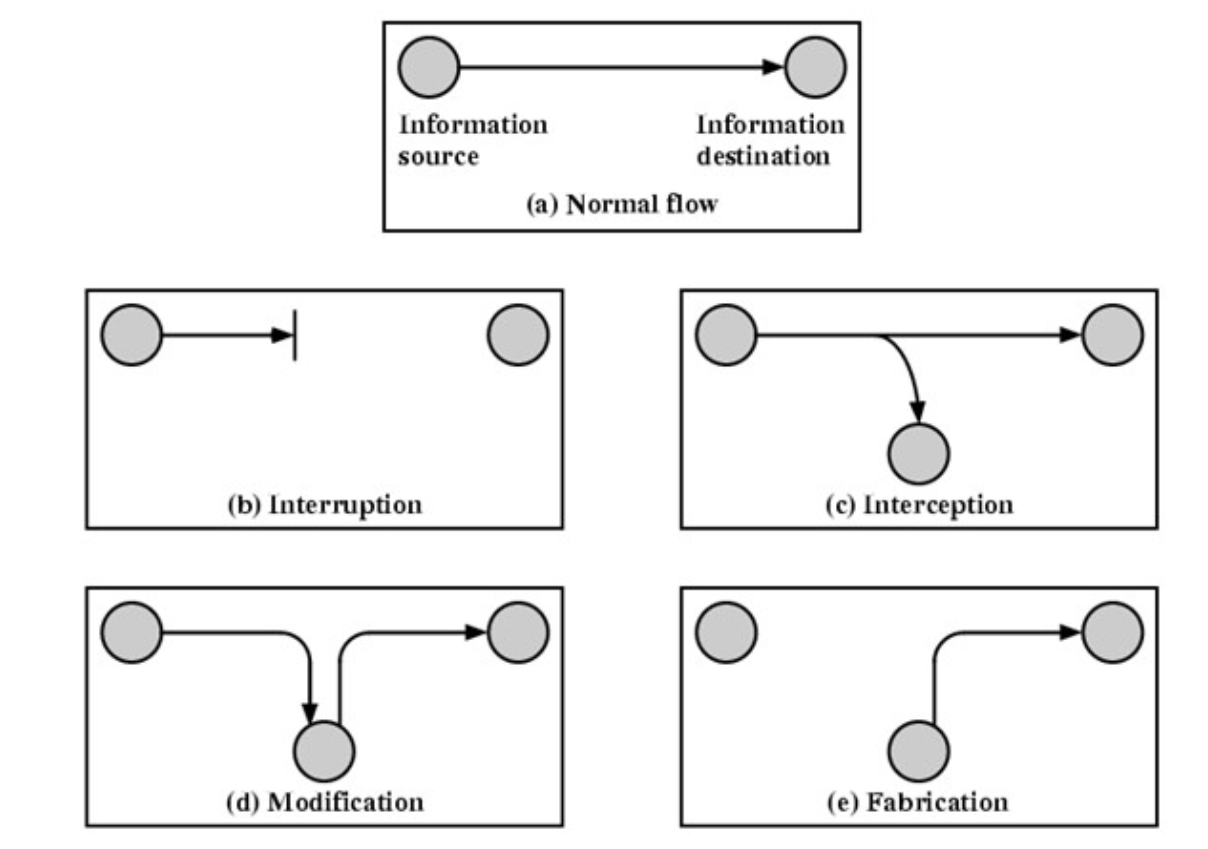
\includegraphics[width=\textwidth]{images/angriffe_pic1.png}
    \caption[Beschriebung für Inhaltsverzeichnis]{Bildbeschreibung} 
    \label{Referenz}
\end{figure} 

\textbf{Unterbrechungen}

Von einer Unterbrechung wird immer dann gesprochen wenn ein Bestandteil des 
IT-Systems zerstört oder unbrauchbar gemacht wird. Die Angriffe zielen darauf 
ab die Verfügbarkeit des betroffenen IT-Systems zu schwächen. 

\textbf{Abfangen}

Die oft als \glqq Man-in-the-middle \grqq{} Angriffe bezeichneten Attacken sind dieser 
Kategorie zuzuweisen. Ein nicht berechtigter Benutzer versucht die Vertrauligkeit des 
IT-Systems zu kompromitieren.  

\textbf{Modifikation}

Von einer Modifikation spricht man immer dann wenn ein Angreifer Zugriff auf einen 
Systemteil gewinnt und auf diesem Daten manipuliert. Diese Angriffsart zielt 
darauf ab die Integrität der Daten zu gefärden. 

\textbf{Fälschung}

Wenn ein Dritter gefälschte Objekte in eine System einschläust spricht man von 
einer Fälschung. Die Fälschung kompromitiert die Authentizität der Daten. 
Ein Beispiel hierfür wäre sogar bereits die Urkundenfälschung auf einem Computersystem. 

Bei der folgenden Betrachtung von Angriffen auf verteilte Systeme werden die Angriffe jeweils einer 
der aufgeführten Kategorien zugeordnet. 

Der bisher wohl bekannteste Cyber-Angriff wurde 2017 in Form der Ransomeware \glqq WannaCry \grqq{} bekannt.
Mithilfe einer Schwachstelle konnte eine Hackergruppe einen sog. Kryptotrojaner über das Netzwerk
auf sehr viele IT-Systeme verteilen. Besonders interessant in dem Zusammenhang mit verteilten Systemen ist 
das Vorgehen des Trojaners in Unternehmen und Institutionen wir bspw. Krankenhäusern. 
In einigen Krankenhäusern wurden alle Geräte, einschließlich Medizinisches Equipment von 
der Schadsoftware verschlüsselt. 
Die Art der Implementierung des Exploits unterschied sich insofern von anderen Verschlüsselungsprogrammen, 
dass der Benutzer keinen Fehler machen musste um betroffen zu sein. 
Der Virus wurde weder durch einen Word Macro, noch einen verdächtigen Link auf den Computer übertragen. 
Besonders bei großen Unternehmen ohne die nötigen Sicherheitsmaßnahmen wurde großer Schaden angerichtet. 
Teilweise musste bei solchen Fällen die Produktion gestoppt werden, was zu einem enormen wirtschaftlichen 
Schaden geführt hat. 
Ein Solcher Angriff ziehlt auf die Komrpomitierung der Verfügbarkeit und Integrität der Daten des 
Zielsystems ab und sorgt somit für eine Unterbrechung- und Modifikation des normalen Datenflusses. 
\\\\
Ein ebenfalls sehr bekanntes Beispiel für einen Cyber-Angriff ist die Malware \glqq Stuxnet. \grqq{}
Das Ziel des Angriffs war es die Leittechnik zur Urananreicherung im Iran außer Kraft zu setzen. 
Dem Wurm war es möglich, sich über USB-Sticks unbemerkt sogar auf Computersysteme ohne Internetzugang 
auszubreiten. Gerieht die Schadsoftware auf einen Rechner der mit einer bestimmten Maschinensteuerung 
verbunden war, programmierte er diese automatisiert um. Das primäre Ziel des Computervirus bestand darin 
die Verfügbarkeit des Zielsystemes zu kompromitieren was zu einer Unterbrechung des normalen Datenflusses führte. 
\\\\
Die Gefahren von Cyberattacken sind sehr umfangreich die hohe Komplexität der Schadsoftware ist der 
Grund warum man nie von einem vollständig sicheren System sprechen kann. 
Von dem Bundesamt für Sicherheit in der Informationstechnik (BSI) sind einige Interessante Fakten darüber veröffentlicht worden: 
\begin{itemize}
    \item Etwa alle zwei Sekunden erscheint ein neues Schadprogramm bzw. eine neue Variante
    \item Pro Minute werden ca. 2 digitale Identitäten in Deutschland gestohlen
    \item Pro Tag werden etwa 4-5 geziehlte Trojaner im Regierungsnetz entdeckt
    \item Pro Monat werden etwa 40.000 Zugriffsversuche aus dem Regierungsnetz auf schädliche Websiten blockiert
\end{itemize}

\section{Anforderungen an verteilte Systeme}


